\documentclass[12pt, titlepage]{article}

\usepackage{fullpage}
\usepackage[round]{natbib}
\usepackage{multirow}
\usepackage{booktabs}
\usepackage{tabularx}
\usepackage{graphicx}
\usepackage{float}
\usepackage{hyperref}

\usepackage[normalem]{ulem}
\usepackage[usenames, dvipsnames]{color}

\hypersetup{
    colorlinks,
    citecolor=black,
    filecolor=black,
    linkcolor=red,
    urlcolor=blue
}
\usepackage[round]{natbib}

\newcounter{acnum}
\newcommand{\actheacnum}{AC\theacnum}
\newcommand{\acref}[1]{AC\ref{#1}}

\newcounter{ucnum}
\newcommand{\uctheucnum}{UC\theucnum}
\newcommand{\uref}[1]{UC\ref{#1}}

\newcounter{mnum}
\newcommand{\mthemnum}{M\themnum}
\newcommand{\mref}[1]{M\ref{#1}}

\title{SE 3XA3: Module Guide\\ DinoDodger}

\author{Team 39, S.R.A Squad
		\\ Razan Abujarad, abujarar
		\\ Shrey Mittal, mittas1
		\\ Zhiwen Yang, yangz18
}

\date{November 10, 2017}

%\input{../../Comments}

\begin{document}

\maketitle

\pagenumbering{roman}
\tableofcontents
\listoftables
\listoffigures

\begin{table}[bp]
\caption{\bf Revision History}
\begin{tabularx}{\textwidth}{p{3cm}p{2cm}X}
\toprule {\bf Date} & {\bf Version} & {\bf Notes}\\
\midrule
\date{2017/11/10} & 1.0 & MG creation\\
\date{2017/12/4} & 2.0 & MG Revision\\
\bottomrule
\end{tabularx}
\end{table}

\newpage

\pagenumbering{arabic}

\section{Introduction}

DinoDodger is a redevelopment of the game T-rex Runner by Chromium. In contrast to the original game, DinoDodger is written in Java, only for PC platforms. This program incorporates design principles such as encapsulation, data hiding and modularity. Refer to the MIS for details on the different modules.\\ \\
The original project was used to determine the requirements for the game along with additional modification unique to DinoDodger. Refer to SRS for documented functional and non-functional requirements. \\ \\


Note: The following paragraph has been used from the template:\\ \\
The documentation is organized as follows : Section \ref{SecChange} lists the anticipated and unlikely changes of the software
requirements. Section \ref{SecMH} summarizes the module decomposition that
was constructed according to the likely changes. Section \ref{SecConnection}
specifies the connections between the software requirements and the
modules. Section \ref{SecMD} gives a detailed description of the
modules. Section \ref{SecTM} includes two traceability matrices. One checks
the completeness of the design against the requirements provided in the SRS. The
other shows the relation between anticipated changes and the modules. Section
\ref{SecUse} describes the use relation between modules.

\section{Anticipated and Unlikely Changes} \label{SecChange}

\subsection{Anticipated Changes} \label{SecAchange}
\begin{description}
\item[\refstepcounter{acnum} \actheacnum \label{ac1}:] The platform is only running on PCs
\item[\refstepcounter{acnum} \actheacnum \label{ac2}:] Spacebar as input for the jumping animation
\item[\refstepcounter{acnum} \actheacnum \label{ac3}:] The usage of the Character module
\item[\refstepcounter{acnum} \actheacnum \label{ac4}:] How different should the characters and landscapes be from each other
\item[\refstepcounter{acnum} \actheacnum \label{ac5}:] Implementing the default selection of the character and landscape
\end{description}

\subsection{Unlikely Changes} \label{SecUchange}
\begin{description}
\item[\refstepcounter{ucnum} \uctheucnum \label{uc1}:] Sprite animation algorithm
\item[\refstepcounter{ucnum} \uctheucnum \label{uc2}:] Changing UI library
\item[\refstepcounter{ucnum} \uctheucnum \label{uc3}:] I/O devices used (Input: Keyboard; Output: Monitor)
\item[\refstepcounter{ucnum} \uctheucnum \label{uc4}:] Programming language that the program used (JavaFX)
\item[\refstepcounter{ucnum} \uctheucnum \label{uc5}:] The options given to user at the end of the game (Restart, Play again, Close)
\end{description}

\section{Module Hierarchy} \label{SecMH}

This section provides an overview of the module design. Modules are summarized
in a hierarchy decomposed by secrets in Table \ref{TblMH}. The modules listed
below, which are leaves in the hierarchy tree, are the modules that will
actually be implemented.

\begin{description}
\item [\refstepcounter{mnum} \mthemnum \label{mUI}:] UI Module
\item  [\refstepcounter{mnum} \mthemnum \label{mDD}:] DinoDodger Module
\item  [\refstepcounter{mnum} \mthemnum \label{mSA}:] SpriteAnimation Module
\textcolor{red}{\item  [\refstepcounter{mnum} \mthemnum \label{mPS}:] PlayScene Module}
\item  [\refstepcounter{mnum} \mthemnum \label{mC}:] Character Module
\textcolor{red}{
\item  [\refstepcounter{mnum} \mthemnum \label{mPT}:] Pterodactyl Module
\item  [\refstepcounter{mnum} \mthemnum \label{mCA}:] Cactus Module 
\item  [\refstepcounter{mnum} \mthemnum \label{mPC}:]  PointCounter}
\end{description}


\begin{table}[h!]
\centering
\begin{tabular}{p{0.3\textwidth} p{0.6\textwidth}}
\toprule
\textbf{Level 1} & \textbf{Level 2}\\
\midrule

\multirow{2}{0.3\textwidth}{Hardware-Hiding Module} 
& \mref{mUI} \\
& \mref{mPS} \\
& \mref{mPC} \\
\midrule

\multirow{3}{0.3\textwidth}{Behaviour-Hiding Module}
 & \mref{mDD}\\
& \mref{mUI} \\
& \mref{mPS} \\
& \mref{mPT} \\
& \mref{mCA} \\
\midrule

\multirow{2}{0.3\textwidth}{Software Decision Module} 
& \mref{mC} \\
& \mref{mSA} \\
\bottomrule

\end{tabular}
\caption{Module Hierarchy}
\label{TblMH}
\end{table}

\section{Connection Between Requirements and Design} \label{SecConnection}
Refer to Table \ref{TblRT}.


\section{Module Decomposition} \label{SecMD}

\subsection{Hardware Hiding Modules}

\begin{description}
\subsubsection{UI Module }
\item[Secrets:] The implementation of the character decision button functionalities as well as theme decision functionalities.
\item[Services:] Determines which character and theme are chosen by the user when the buttons are clicked.
\item[Implemented By:] OS

\textcolor{red}{\subsubsection{PointCounter}}
\textcolor{red}{\item[Secrets:] The implementation of the algorithm that determines the score of the user.}
\textcolor{red}{\item[Services:] Counts the users score as long as the game is running.} 


\end{description}

\subsection{Behaviour-Hiding Module}
\begin{description}

\subsubsection{Character Module}
\item[Secrets:] The implementation of the JUMP method and makes use of the Sprite Animation.
\item[Services:] Allows the user to make the character jump to avoid obstacles.


\textcolor{red}{
\subsubsection{Pterodactyl Module}
\item[Secrets:] The implementation of the Pterodactyl obstacle objects.
\item[Services:] Generates pterodactyl obstacles at random time intervals.
\subsubsection{Cactus}
\item[Secrets:] The implementation of the algorithm that generates a random number/size of cacti.
\item[Services:] Generates randomly sized cacti obstacles at random intervals. }

\subsubsection{PlayScene Module}
\item[Secrets:] The implementation of the background motion including the ground element, cloud element and cacti elements.
\item[Services:] Allows the background of the game scene to move in synchronization with the character. This module allows the user to view the obstacles and allows the user to provide a response to overcome the obstacles.

\subsubsection{Sprite Animation Module}
\item[Secrets:] The implementation of the character's movement animation i.e the way in which the character moves through the game and the motion of the characters legs.
\item[Services:] Allows the character to seem to be running such that the user can understand that the character is moving if the game is running.

\end{description}

\subsection{Input Format Module - UI Module}
\begin{description}
\item[Secrets:] The algorithm that converts the buttons clicked by the user to a character selection.
\item[Services:] Converts the users input from the UI buttons to character selection by reading the button values corresponding to specific characters.
\end{description}

\subsection{Software Decision Module}
\begin{description}

\subsubsection{DinoDodger}
\item[Secrets:] Implementation of the message passing between UI to Animation modules.
\item[Services:] This module allows the communication between the UI module where the user inputs data and the Animation module where the user views and manipulates the character. 
This module does not interact with the user but with other modules to bring the game together.
\end{description}


\section{Traceability Matrix} \label{SecTM}

This section shows two traceability matrices: between the modules and the
requirements and between the modules and the anticipated changes. \\

Refer to \textcolor{red}{Section 2 in the} SRS for requirements and Section \ref{SecAchange} for anticipated changes.

\begin{table}[H]
\centering
\begin{tabular}{p{0.2\textwidth} p{0.6\textwidth}}
\toprule
\textbf{Req.} & \textbf{Modules}\\
\midrule
2.2.1 & \mref{mUI}\\
2.2.2 & \mref{mUI} \\
2.2.3 & \mref{mUI}\\
2.2.4 & \mref{mUI}, \mref{mPS}\\
2.2.5 & \mref{mPS}, \mref{mC} \\
2.2.6 & \mref{mPS}, \mref{mUI}\\
2.2.7 & \mref{mUI}\\
2.2.8 & \mref{mPS} \\
2.2.9 & \mref{mPS}, \mref{mC} \\
2.2.10 & \mref{mCA} \\
2.2.11 & \mref{mPS} \\
2.2.12 & \mref{mPS} \\
2.2.13 & \mref{mPS} \\
2.2.14 & \mref{mPS}, \mref{mUI} \\
2.2.15 & \mref{mPS} \\
2.2.16 & \mref{mUI} \\
2.2.17 & \mref{mUI} \\
2.2.18 & \mref{mUI} \\
2.2.19 & \mref{mUI} \\
2.2.20 & \mref{mUI} \\
2.2.21 & \mref{mPC} \\
2.2.22 & \mref{mPT} \\
\bottomrule
\end{tabular}
\caption{Trace Between Requirements and Modules}
\label{TblRT}
\end{table}

\begin{table}[H]
\centering
\begin{tabular}{p{0.2\textwidth} p{0.6\textwidth}}
\toprule
\textbf{AC} & \textbf{Modules}\\
\midrule
\acref{ac1} & \mref{mUI}\\
\acref{ac2} & \mref{mPS}\\
\acref{ac3} & \mref{mC}, \mref{mPS}\\
\acref{ac4} & \mref{mUI}, \mref{mPS}\\
\acref{ac5} & \mref{mUI}, \mref{mDD}\\
\bottomrule
\end{tabular}
\caption{Trace Between Anticipated Changes and Modules}
\label{TblACT}
\end{table}

\section{Use Hierarchy Between Modules} \label{SecUse}
A Uses Hierarchy exists between the modules such that :
\begin{itemize}
\item {\sout{DinoDodger module uses  Module and UI module}}
\item {\sout{Animation module uses the Character module}}
\item {\sout{Character module uses the Sprite Animation module.}} 
\end{itemize}  

\begin{itemize}
\item{\textcolor{red}{ UI module uses PlayScene module}}
\item{\textcolor{red}{UI module uses DinoDodger module}} 
\item{\textcolor{red}{PlayScene module uses Pterodactyl, Character and Cactus modules}}
\item{\textcolor{red}{PlayScene module uses PointsCounter module}}
\item{\textcolor{red}{PlayScene module uses DinoDodger module}}
\item{\textcolor{red}{Character and Pterodactyl modules use the SpriteAnimation module}}
\item{\textcolor{red}{Cactus module uses DinoDodger module}}
\end{itemize}

\begin{figure}[H]
\centering
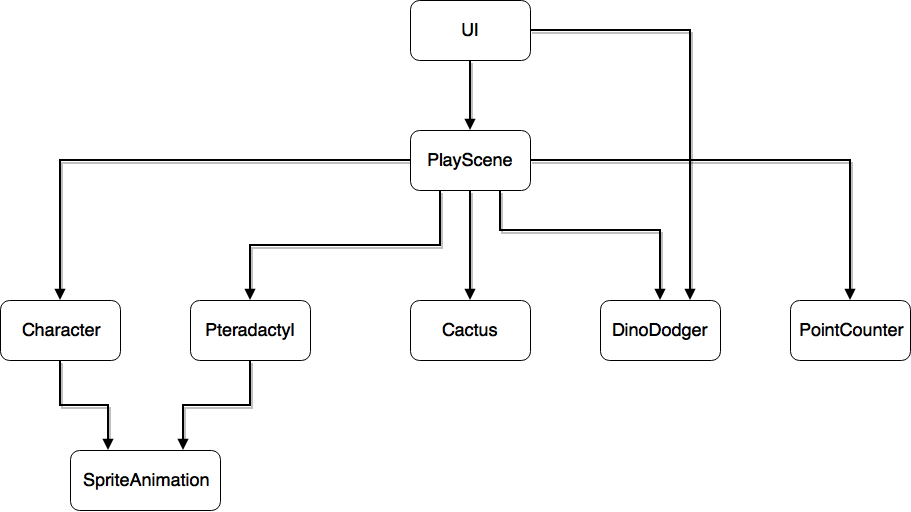
\includegraphics[width=0.7\textwidth]{USES.png}

\caption{Use hierarchy among modules}
\label{FigUH}
\end{figure}

\bibliographystyle {plainnat}
\bibliography {MG}

\end{document}
